%%%%%%%%%%%%%%%%%%%%%%%%%%%%%%%%%%%%%%%%%
% Beamer Presentation
% LaTeX Template
% Version 1.0 (10/11/12)
%
% This template has been downloaded from:
% http://www.LaTeXTemplates.com
%
% License:
% CC BY-NC-SA 3.0 (http://creativecommons.org/licenses/by-nc-sa/3.0/)
%
%%%%%%%%%%%%%%%%%%%%%%%%%%%%%%%%%%%%%%%%%

%----------------------------------------------------------------------------------------
%	PACKAGES AND THEMES
%----------------------------------------------------------------------------------------

\documentclass[10pt]{beamer}
%\documentclass[handout, 10pt]{beamer}
\setbeamercovered{transparent}

\mode<presentation> {

% The Beamer class comes with a number of default slide themes
% which change the colors and layouts of slides. Below this is a list
% of all the themes, uncomment each in turn to see what they look like.

%\usetheme{default}
%\usetheme{AnnArbor}
%\usetheme{Antibes}
%\usetheme{Bergen}
%\usetheme{Berkeley} % Neat Contents on left
%\usetheme{Berlin}
%\usetheme{Boadilla}
%\usetheme{CambridgeUS} % Neat but breadcrumbs at top
%\usetheme{Copenhagen}
%\usetheme{Darmstadt}
%\usetheme{Dresden}
%\usetheme{Frankfurt}
%\usetheme{Goettingen} %Neat contents on right
%\usetheme{Hannover} %Neat contents on left
%\usetheme{Ilmenau}
%\usetheme{JuanLesPins}
%\usetheme{Luebeck}
%\usetheme{Madrid}
%\usetheme{Malmoe}
%\usetheme{Marburg} % Contents on right in contrast color
%\usetheme{Montpellier}
\usetheme{PaloAlto} % Contents on left
%\usetheme{Pittsburgh}
%\usetheme{Rochester}
%\usetheme{Singapore}
%\usetheme{Szeged}
%\usetheme{Warsaw}

% As well as themes, the Beamer class has a number of color themes
% for any slide theme. Uncomment each of these in turn to see how it
% changes the colors of your current slide theme.

%\usecolortheme{albatross}
%\usecolortheme{beaver}
%\usecolortheme{beetle}
%\usecolortheme{crane}
%\usecolortheme{dolphin}
%\usecolortheme{dove}
%\usecolortheme{fly}
%\usecolortheme{lily}
%\usecolortheme{orchid}
%\usecolortheme{rose}
\usecolortheme{seagull}
%\usecolortheme{seahorse}
%\usecolortheme{whale}
%\usecolortheme{wolverine}

%\setbeamertemplate{footline} % To remove the footer line in all slides uncomment this line
%\setbeamertemplate{footline}[page number] % To replace the footer line in all slides with a simple slide count uncomment this line

%\setbeamertemplate{navigation symbols}{} % To remove the navigation symbols from the bottom of all slides uncomment this line
}

\usepackage{graphicx} % Allows including images
\usepackage{booktabs} % Allows the use of \toprule, \midrule and \bottomrule in tables

%----------------------------------------------------------------------------------------
%	TITLE PAGE
%----------------------------------------------------------------------------------------

\title[Improving Outcomes in Pancreatic Surgery]{An investigation of the clinical utility of preoperative cardiopulmonary exercise testing in patients undergoing major pancreatic surgery.} % The short title appears at the bottom of every slide, the full title is only on the title page

\author{Vishnu V Chandrabalan} % Your name
\institute[UoG] % Your institution as it will appear on the bottom of every slide, may be shorthand to save space
{
University of Glasgow \\ % Your institution for the title page
\medskip
% \textit{john@smith.com} % Your email address
}
\date{\today} % Date, can be changed to a custom date

\begin{document}

\begin{frame}
\titlepage % Print the title page as the first slide
\end{frame}

%\begin{frame}
%	\frametitle{My Supervisors - Thank you!}
%	I wish to thank the following people for their unwavering support through the past few years. I thank them especially for their faith that I will see this through and if they had any doubts, for not telling me about them.\\
%	\bigskip
%	Professor Donald C McMillan,\\
%	University Department of Surgery, Glasgow Royal Infirmary\\
%	\bigskip
%	Professor Paul Horgan,\\
%	University Department of Surgery, Glasgow Royal Infirmary\\
%\end{frame}

\begin{frame}
\frametitle{Overview} % Table of contents slide, comment this block out to remove it
\tableofcontents % Throughout your presentation, if you choose to use \section{} and \subsection{} commands, these will automatically be printed on this slide as an overview of your presentation
\end{frame}

%----------------------------------------------------------------------------------------
%	PRESENTATION SLIDES
%----------------------------------------------------------------------------------------

%------------------------------------------------
%\section{Chapter 1/ Introduction}
\section[Chapter 1]{Introduction}

\begin{frame}
	\frametitle{Pancreatic cancer} %Epidemiology/outcomes
	\begin{block}{The Problem}
		\begin{itemize}
			\item 10th common but 5th common cause of cancer death
			\item Survival	1-yr: 20.8\%, 5-yr: 3.3\%, 10yr: 1.1\%
			\item Operable disease : approx 15\%
		\end{itemize}
	\end{block}
	\begin{block}{Treatment}
		\begin{itemize}
			\item Surgery + adjuvant chemotherapy only chance of cure
		\end{itemize}
	\end{block}
	\begin{block}{Pancreaticoduodenectomy}
		\begin{itemize}
			\item Complex surgery with 40\% morbidity
			\item Performed only in specialist centres
			\item Patient fitness is as important as tumour factors
			\item Adjuvant treatment improves survival
		\end{itemize}
	\end{block}
\end{frame}

\begin{frame}
	\frametitle{Pancreaticoduodenectomy}
	\framesubtitle{Postoperative complications}
	\begin{itemize}
		\item Significant improvements in mortality ($<$5\% from $>$40\%)
		\item Morbidity remains high at over 40\%
		\item Postoperative pancreatic fistula (POPF) is serious
		\item POPF can lead to other complications: Sepsis, PPH, DGE
		\item International Study Group for Pancreatic Surgery
		\item Clavien-Dindo classification of complications
		\medskip
		\item Complications may preclude adjuvant treatment
		\item Median survival is approximately 18 months
		\item Adjuvant treatment improves this by 2-3 months
	\end{itemize}
\end{frame}

\begin{frame}
	\frametitle{Risk Stratification }
	\framesubtitle{Section 1.4 Pages 13-18 }
	\begin{itemize}
		\item Patient fitness is important determinant of outcome
		\item Effect of comorbidity on function is difficult to assess
		\item POSSUM, APACHE, mGPS, E-PASS, etc.
		\item Static measures do not predict performance under stress
		\item Do not provide targets for prehabilitation
		\item Preoperative management of obstructive jaundice remains controversial
		\item Pancreas specific risk factors of POPF
		\begin{itemize}
			\item Soft pancreas, narrow pancreatic duct, non-obstructing pathology
			\item These factors are not modifiable
			\item Coronary artery disease! (Lin 2004)
		\end{itemize}
	\end{itemize}
\end{frame}

\begin{frame}
	\frametitle{Cardiopulmonary exercise testing}
	\framesubtitle{What, how, why?}
	{\footnotesize
	\begin{itemize}
		\item Objective measure of cardiopulmonary response to exercise
		\item Dynamic test measuring multiple aspects of oxygen delivery
		\item Cardiac, respiratory, vascular and mitochondrial function
		\item First described for preoperative assessment by Older and co-workers
		\item Widely used in general, oesophago-gastric, vascular and thoracic surgery
	\end{itemize}
	\vfill

	\begin{columns}
		\column[c]{0.6\textwidth}
			\textbf{CPET Methodology}
			\\ - Cycle ergometer with electronic braking
			\\ - Breath-by-breath gas analysis
			\\ - 12-lead ECG monitoring
			\\ - Initial 3-minute rest for baseline
			\\ - Incremental load to volitional fatigue
				
		\column[c]{0.4\textwidth}

			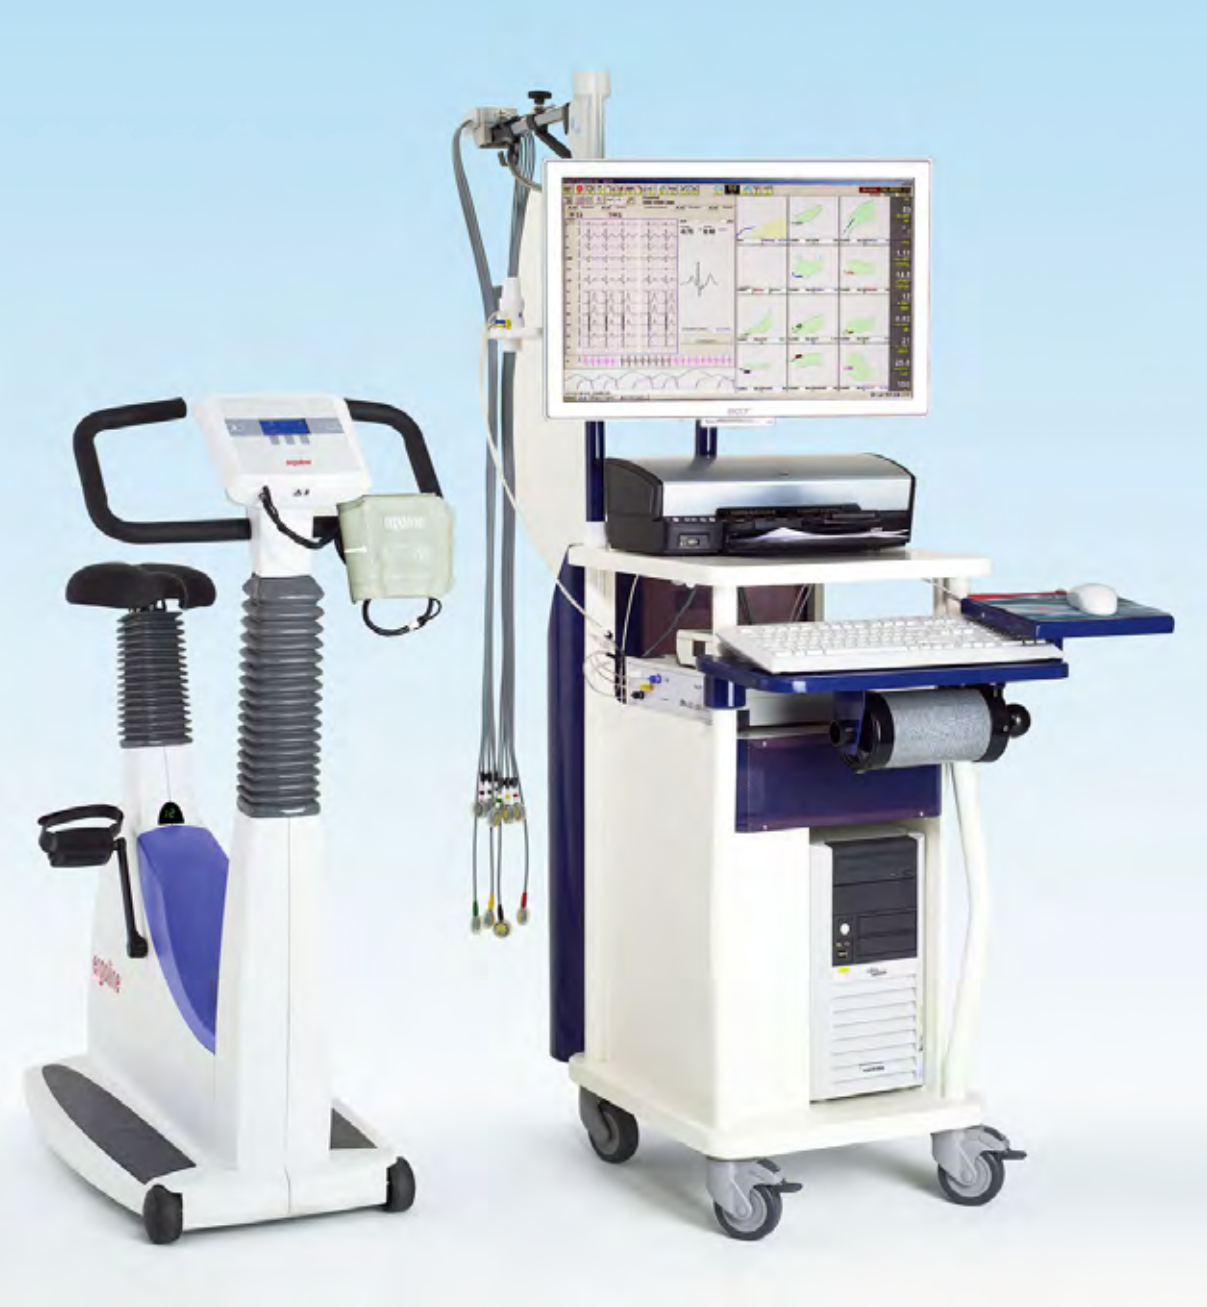
\includegraphics[height=0.4\textheight]{../Figures/cpet-zan}


		
	\end{columns}
	}
\end{frame}

\begin{frame}
	\frametitle{Physiological basis of CPET} 
	\begin{columns}
	\column[c]{0.5\textwidth}

		\begin{figure}
			\includegraphics[width=\linewidth]{CellRespiration}
		\end{figure}
		{\scriptsize $H^+ + HCO3^- \Longleftrightarrow H_2CO_3 \Longleftrightarrow H_2O + CO_2$}

	\column[c]{0.5\textwidth}
	\begin{figure}[htbp]
		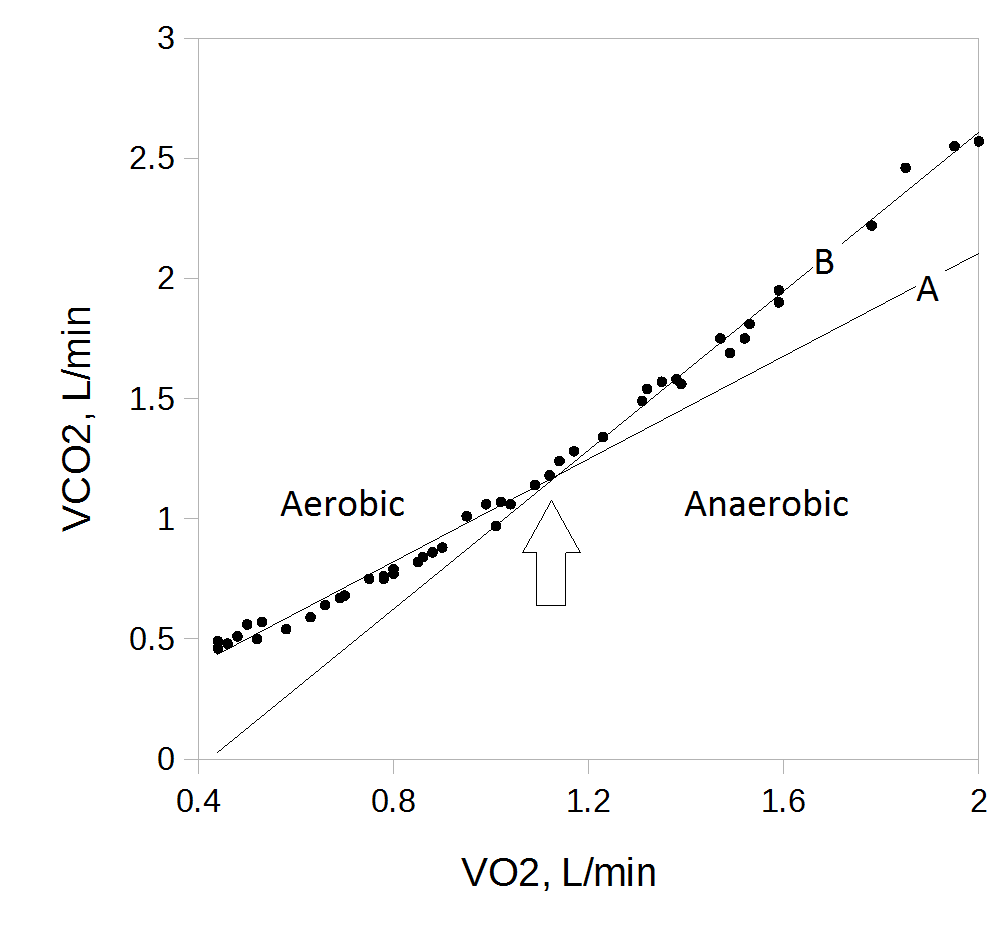
\includegraphics[width=\linewidth]{../Figures/cpet_vslope}
	\end{figure}
	
	\end{columns}

\end{frame}

\begin{frame}
	\frametitle{Aims of Thesis}
	\begin{enumerate}
		\item To evaluate the clinical utility of preoperative CPET in predicting postoperative adverse events after pancreaticoduodenectomy.
\pause
		\item To examine the patient factors that are related to cardiopulmonary exercise physiology with particular attention to the effect of obstructive jaundice and body composition.
\pause
		\item To examine the effect of preoperative systemic inflammation and poor aerobic capacity on the magnitude of the post-operative systemic inflammatory response.
\pause
		\item To examine the value of serial daily postoperative markers of systemic inflammatory response in the prediction of post-operative complications.
	\end{enumerate}
\end{frame}



%--CHAPTER 2----CHAPTER 2----CHAPTER 2----CHAPTER 2----CHAPTER 2----CHAPTER 2----CHAPTER 2--
\section[Chapter 2]{CPET and Postoperative Outcomes}
\begin{frame}
	\frametitle{CPET and Postoperative Outcomes}
	\framesubtitle{Does CPET have a role in risk stratification of patients?}
	\begin{block}{\textbf{Complications}}
		Low $\dot{V}_{O_2}$AT associated with pancreatic fistula (16\% vs 35\%) \\
		Not associated with cardio-respiratory complications or mortality
	\end{block}
\pause	
	\begin{block}{\textbf{Length of stay}}
		Low $\dot{V}_{O_2}$AT associated with longer hospital stay (14 vs 20 days)\\
		Not associated with critical care stay or admissions
	\end{block}
\pause	
	\begin{block}{\textbf{Adjuvant Therapy}}
		Low $\dot{V}_{O_2}$AT associated with non-progression to adjuvant therapy after surgery.
	\end{block}
\end{frame}

\begin{frame}
	\frametitle{CPET in the Glasgow Cohort}
	\framesubtitle{Why was 'aerobic capacity' so poor in these patients, yet outcomes were comparable?}
	\begin{figure}
		\centering
		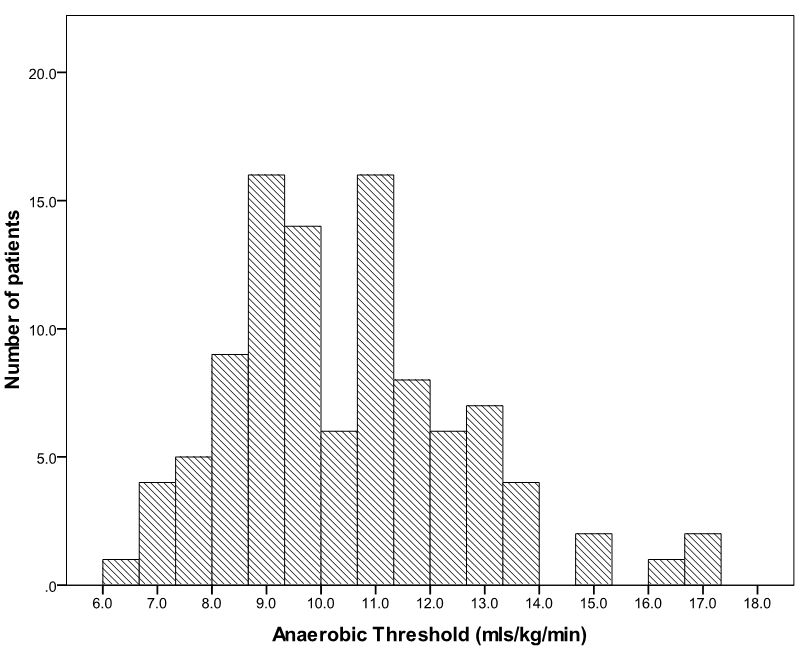
\includegraphics[height=0.35\textheight]{../Figures/cpet_outcomes_dist_of_AT}
	\end{figure}

	\begin{itemize}
		\item Median AT = 10.3 ml/kg/min (IQR 8.8 -11.6)
		\item $\dot{V}_{O_2}$AT$<$10 ml/kg/min in 49\% of patients
		\item Different from other cohorts
		\item $\dot{V}_{O_2}AT<11$ ml/kg/min in
		\begin{itemize}
			\item 16\% undergoing oesophageal surgery [Forshaw 2008]
			\item 39\% undergoing liver transplantation [Epstein 2004]
			\item 29\% undergoing abdominal surgery [Older 1993]
		\end{itemize}
	\end{itemize}
\end{frame}

\begin{frame}
	\frametitle{CPET and Postoperative Outcomes}
	\framesubtitle{Publication, Citations and more questions!}
	
	\begin{figure}
		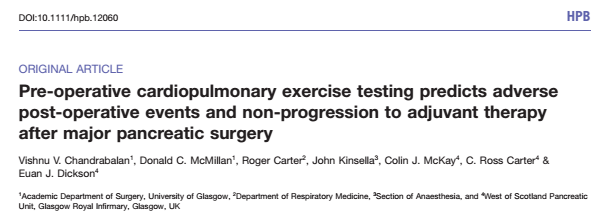
\includegraphics[width=0.6\linewidth]{cpet_hpb_publication}
	\end{figure}

	\begin{columns}[c]
		\column{0.4\textwidth}
			\begin{figure}
				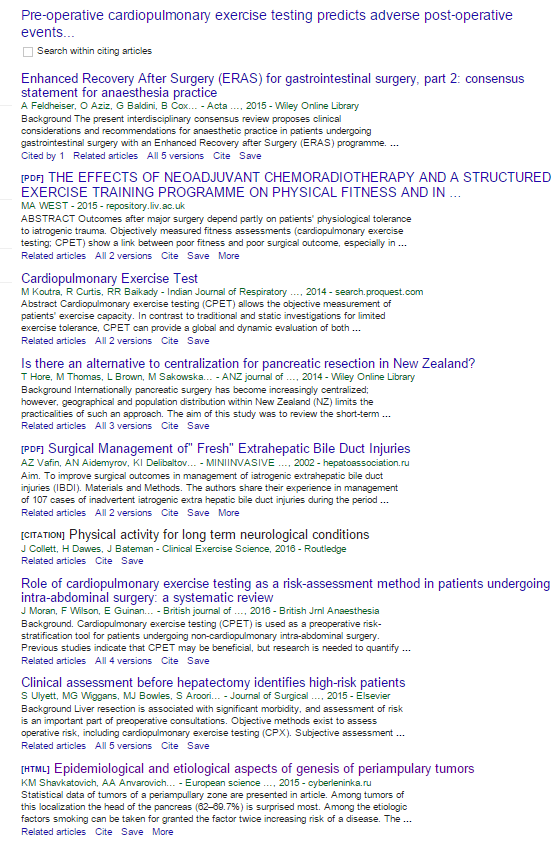
\includegraphics[width=0.6\textwidth]{cpet_citations}
			\end{figure}
	
		\column{0.6\textwidth}
\pause
			{\footnotesize 	Why is $\dot{V}_{O_2}$AT so low in patients undergoing pancreatic surgery?\\
				\medskip

				What factors are associated with a low $\dot{V}_{O_2}$AT?\\
				\medskip
\pause
				Why was $\dot{V}_{O_2}$AT not associated with cardio-respiratory complications?\\
				\medskip

				Does $\dot{V}_{O_2}$AT truly reflect cardiopulmonary function in this cohort of patients?\\	
			}
			
	\end{columns}
\end{frame}


%--CHAPTER 3----CHAPTER 3----CHAPTER 3----CHAPTER 3----CHAPTER 3----CHAPTER 3----CHAPTER 3--
\section[Chapter 3]{CPET, Jaundice and Preoperative Pathophysiology}

\begin{frame}
	\frametitle{What was the effect of jaundice on $\dot{V}_{O_2}$?}
	\framesubtitle{None on multivariate analysis. Weak correlation on scatter-plot analysis.}
	\begin{columns}[t]
		\column{0.5\textwidth}
		\begin{figure}
			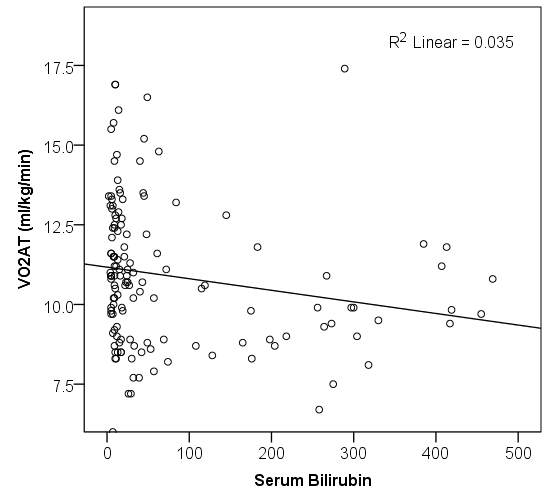
\includegraphics[width=\textwidth]{../Figures/cpet_oj_scatter_at_bil}
			\\ $\dot{V}_{O_2}$AT versus serum bilirubin
		\end{figure}
		
		\column{0.5\textwidth}
		\begin{figure}
			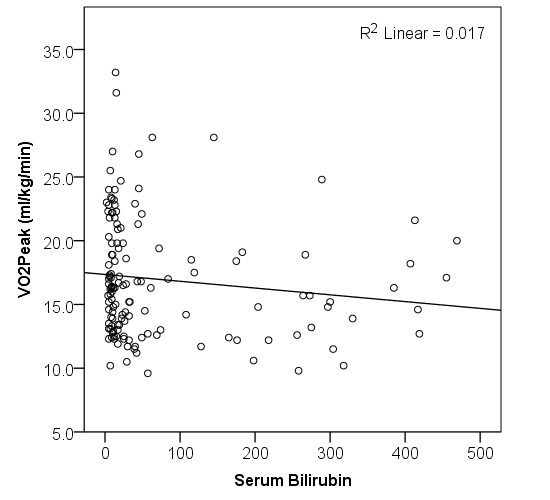
\includegraphics[width=\textwidth]{../Figures/cpet_oj_scatter_peak_bil}
			\\ $\dot{V}_{O_2}$Peak versus serum bilirubin
		\end{figure}
	\end{columns}
\end{frame}

\begin{frame}
	\frametitle{Jaundice and other patient characteristics}
	\framesubtitle{What was the relationship between obstructive jaundice and other parameters?}
	
	\begin{columns}
		\column[c]{0.5\textwidth}		
		
		\begin{figure}
			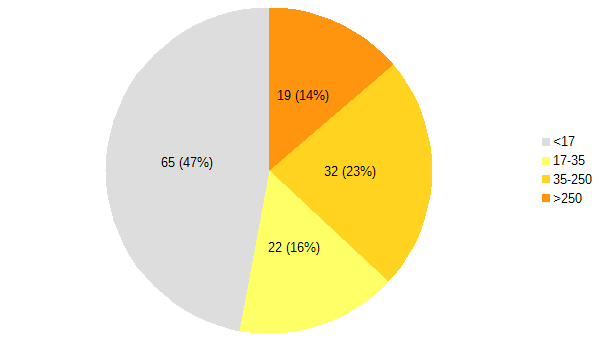
\includegraphics[width=\textwidth]{jaundice_distribution}
		\end{figure}
		
		\begin{figure}
			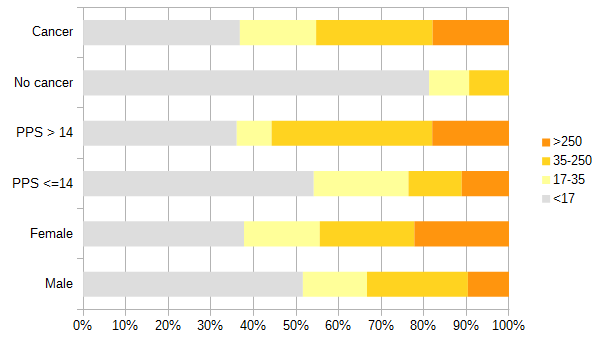
\includegraphics[width=\textwidth]{jaundice_vs_patient_factors}
		\end{figure}
		\pause		
		\column[c]{0.5\textwidth}		
		{\scriptsize			
			Severity of systemic inflammation proportionate to severity of jaundice. \\
			\medskip
			Obstructive jaundice associated with electrolyte abnormalities.\\
			\medskip
			Jaundiced patients were more likely to be anaemic, with lower haematocrit and lower mean corpuscular volume.\\
			\medskip
			No significant difference in the preoperative renal function, prothrombin time and white cell count between jaundiced and non-jaundiced patients.\\
		}
	\end{columns}
\end{frame}


\begin{frame}
	\frametitle{What preop factors were associated with low $\dot{V}_{O_2}$?}
	\framesubtitle{Multivariate binary logistic regression analysis}
	Factors associated with $\dot{V}_{O_2}$AT $<$ 10 ml/kg/min
	\begin{table}
		\begin{tabular}{l| l l l}
			& HR   & 95\% CI    & p     \\ \hline
			Female sex & 3.75 & 1.57-8.95  & 0.003 \\
			BMI$>$25   & 3.65 & 1.61-8.26  & 0.002 \\
			Cancer     & 4.02 & 1.33-12.16 & 0.014 \\
			CRP$>$10   & 2.98 & 1.29-6.86  & 0.010
		\end{tabular}
	\end{table}
	\hrule
\pause
	\medskip
	Factors associated with $\dot{V}_{O_2}$Peak $<$ 16ml/kg/min
	\begin{table}
		\begin{tabular}{l| l l l}
			& HR   & 95\% CI   & p        \\ \hline
			Female sex  & 7.57 & 3.09-18.5 & $<$0.001 \\
			BMI$>$25    & 2.57 & 1.18-5.63 & 0.018    \\
			Haemoglobin & 2.43 & 1.05-5.63 & 0.038
		\end{tabular}
	\end{table}
\end{frame}



%--CHAPTER 4----CHAPTER 4----CHAPTER 4----CHAPTER 4----CHAPTER 4----CHAPTER 4----CHAPTER 4--
\section[Chapter 4]{CPET and Body Composition}

\begin{frame}
	\frametitle{ CPET and Body Composition}
	\framesubtitle{What causes a low $\dot{V}_{O_2}$? }
	\begin{itemize}
		\item Low $\dot{V}_{O_2}$ has been universally ascribed to low aerobic fitness due to inadequate cardio-pulmonary reserve
		\item Occassionally anaemia, peripheral vascular disease or even mitochondrial diseases may play a role
		\item $\dot{V}_{O_2}$AT and $\dot{V}_{O_2}$Peak are most commonly used parameters
		\item During exercise $\dot{V}_{O_2}$ is a function of skeletal muscle mass
		\item But, both are normalised by against patient's total body weight
		\item 'Spurious correlation' unfairly penalises obese subjects
		\item Most patients in this cohort did not have overt cardiac/respiratory disease that could explain the low $\dot{V}_{O_2}$.
	\end{itemize}
\end{frame}

\begin{frame}
	\frametitle{Corrected $\dot{V}_{O_2}$ vs. Absolute $\dot{V}_{O_2}$}
	\framesubtitle{Could this be a source of spurious correlation?}
	
	\[Corrected\ \dot{V}_{O_2} (ml/kg/min) = \frac{Absolute\ \dot{V}_{O_2}\ (litres/min) * 1000}{Total\ body\ weight\ (kg)}\]

	\vfill
\pause	
	For example, if the absolute $\dot{V}_{O_2}$AT was 0.84 litres/min, the corrected $\dot{V}_{O_2}$AT (ml/kg/min) would vary with patient weight as follows:
	
	\begin{table}
	\begin{tabular}{c c c c c c}
		     Weight       & kg        & 70 & 80   & 90  & 100 \\
		$\dot{V}_{O_2}$AT & ml/kg/min & 12 & 10.5 & 9.3 & 8.4
	\end{tabular}
	\end{table}


\end{frame}

\begin{frame}
	\frametitle{Body composition differences between the sexes}
	\framesubtitle{Significant differences in skeletal muscle area across all BMIs.}
	\begin{figure}
		\centering
		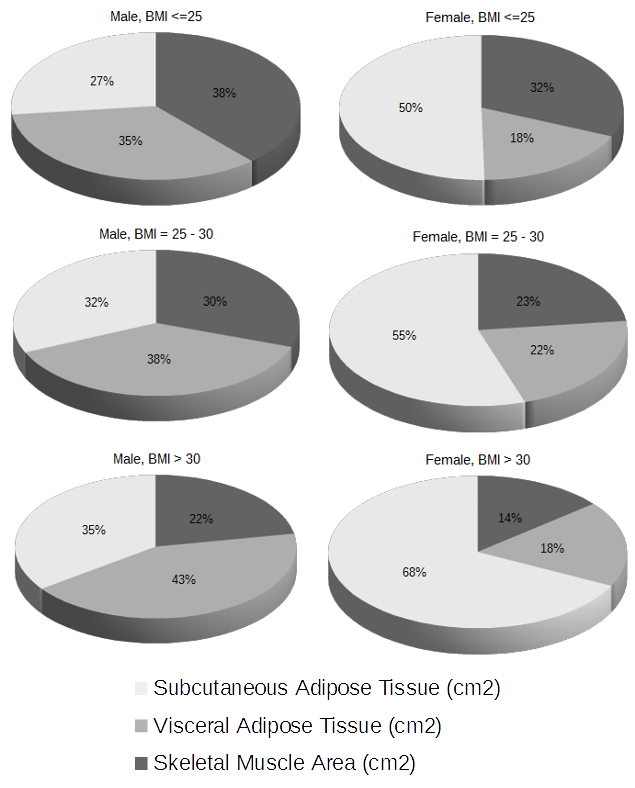
\includegraphics[height=0.95\textheight]{../Figures/bc_gender_bmi_pie}
		\label{fig:bc_gimp}
	\end{figure}
\end{frame}

\begin{frame}
	\frametitle{$\dot{V}_{O_2}$AT vs Total Adipose Tissue}
	\framesubtitle{Figure 4.4(B) Page 111, Figure 4.5(B) on Page 114}
	
	\begin{figure}
		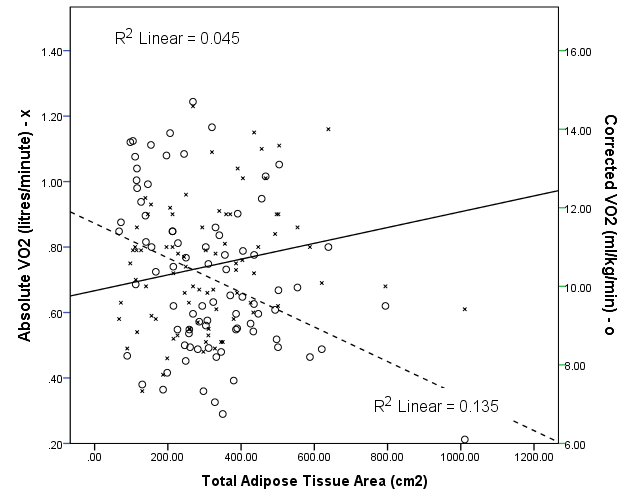
\includegraphics[height=0.4\textheight]{../Figures/bc_scatter_VO2_TAT}
	\end{figure}

	\begin{figure}
		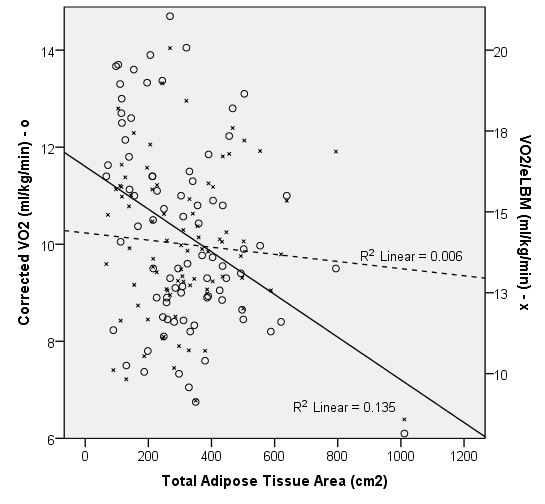
\includegraphics[height=0.45\textheight]{../Figures/bc_scatter_VO2_TAT_elbm}
	\end{figure}
	
\end{frame}

\begin{frame}
	\frametitle{$\dot{V}_{O_2}$AT vs Skeletal Muscle}
	\framesubtitle{Figure 4.4(A) Page 111, Figure 4.5(A) on Page 114}


	\begin{figure}
		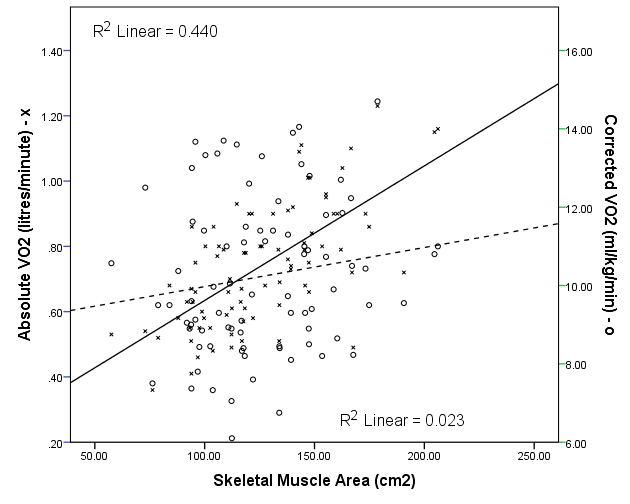
\includegraphics[height=0.4\textheight]{../Figures/bc_scatter_VO2_skeletal}
	\end{figure}

	\begin{figure}
		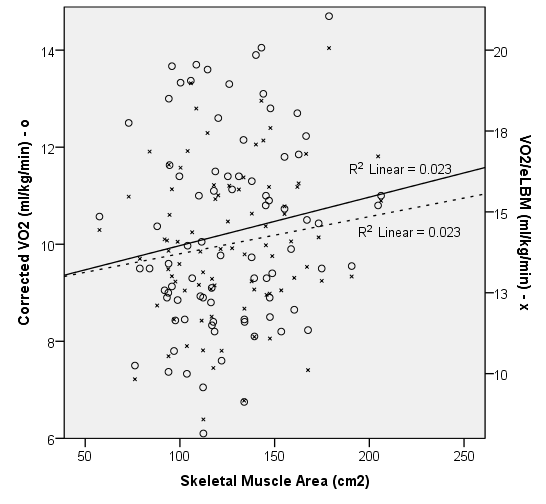
\includegraphics[height=0.45\textheight]{../Figures/bc_scatter_VO2_skeletal_elbm}
	\end{figure}
	
\end{frame}

\section[Chapter 5]{Factors affecting post op inflammation}

\begin{frame}
	\frametitle{Impact of perioperative systemic inflammation?}
	\framesubtitle{Inflammation before and after surgery affects short and long term outcomes}
	\begin{itemize}
		\item Perioperative systemic inflammation affects short and long-term outcomes
		\item Elevated preoperative systemic inflammation is associated with postoperative complications in colorectal surgery, after oesophagectomy, liver resections and cardiac surgery. 
		\item Early exaggerated postoperative systemic inflammatory response is also associated with increased infective complications
		\item In patients undergoing pancreatic surgery, preoperative inflammatory state is further influenced by:
		\begin{itemize}
			\item Obstructive jaundice
			\item Cholangitis
			\item ERCP and stenting
			\item Post-ERCP / EUS related complications
		\end{itemize}
		\item Obesity is associated with chronic inflammation
		\item Impact of aerobic capacity on postoperative inflammation not studied before
	\end{itemize}
\end{frame}

\begin{frame}
	\frametitle{Preop inflammation vs. Postop CRP}
	\framesubtitle{Post op CRP trends are influenced by both preop CRP and preop albumin.}
	\begin{figure}
		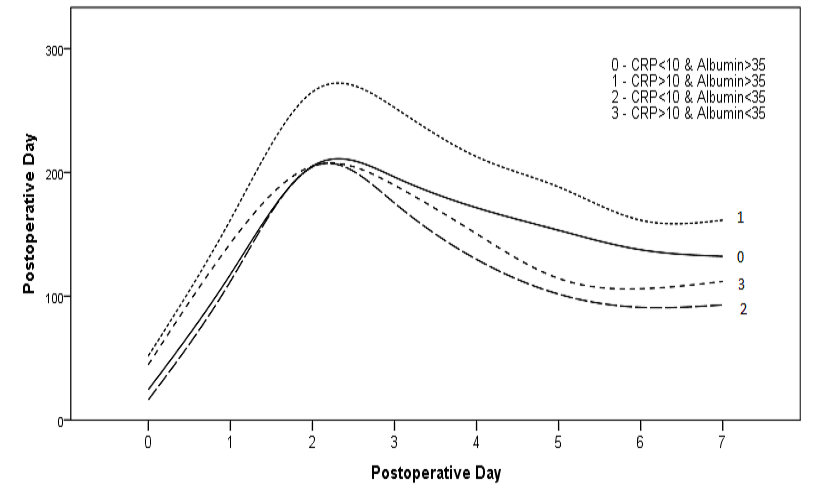
\includegraphics[width=\textwidth]{../Figures/sirs_crp_crp_alb}
	\end{figure}
\end{frame}

\begin{frame}
	\frametitle{Obstructive jaundice vs. Postop CRP}
	\framesubtitle{Obstructive jaundice is associated with an attenuated inflammatory response.}
	\begin{figure}
		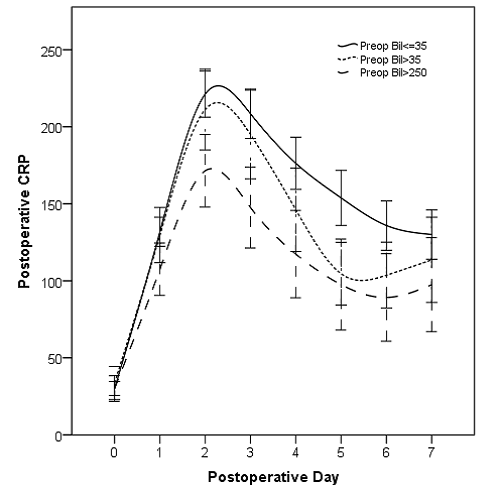
\includegraphics[width=0.7\textwidth]{../Figures/sirs_bil_crp}
	\end{figure}

\end{frame}

\begin{frame}
	\frametitle{CPET, Body composition vs. Postop Inflammation }
	\framesubtitle{Section 5.3.4, 5.3.5 Pages 132-133, Tables 5.8-5.10 Pages 145-147 }
	\begin{itemize}
		\item No relationship between $\dot{V}_{O_2}$ and post op. CRP or neutrophil count
		\vfill
		\item Serum albumin levels lower in patients with low VO2
		\begin{itemize}
			\item Probably related to preop hypoalbuminemia
			\item This in turn related to low skeletal muscle and multiple other factors
		\end{itemize}
		\vfill
		\item No relationship between body composition and postoperative CRP/neutrophil counts
	\end{itemize}
\end{frame}


\section[Chapter 6]{Postoperative CRP and complications}

\begin{frame}
	\frametitle{Does post op. CRP predict severity of POPF?}
	\framesubtitle{No, it does not. \\ Moreover, diagnosis of POPF is made on the third day using drain amylase. }
	
	\begin{columns}
		\column[c]{0.45\textwidth}
			\begin{figure}
				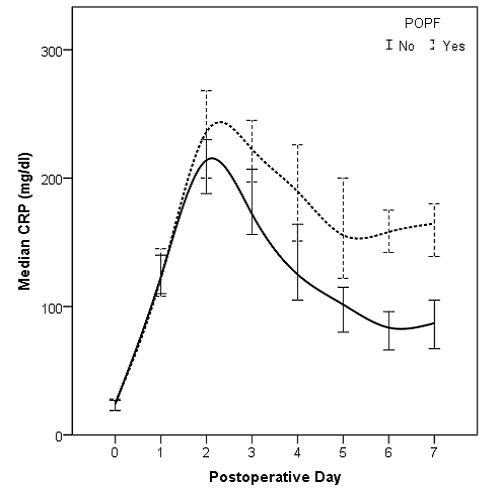
\includegraphics[width=\textwidth]{../Figures/crp_comp_crp_popf_yes_no}
			\end{figure}
	
		\column[c]{0.45\textwidth}
			\begin{figure}
				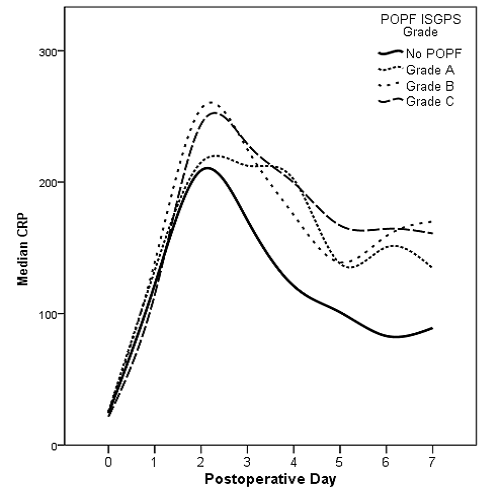
\includegraphics[width=\textwidth]{../Figures/crp_comp_crp_popf_isgps}
			\end{figure}
	\end{columns}

\end{frame}

\begin{frame}
	\frametitle{Does post op. CRP predict infective complications?}
	\framesubtitle{Yes, it does. \\ But, only in the absence of a pancreatic fistula. }
	
	\begin{columns}
		\column[c]{0.45\textwidth}
		\begin{figure}
			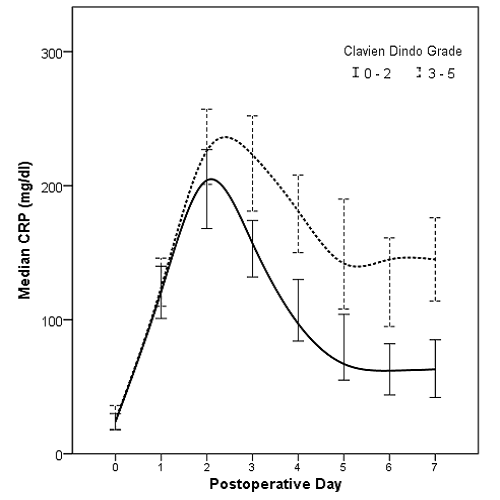
\includegraphics[width=\textwidth]{../Figures/crp_comp_infective_leak0}
			\\ Patients with NO POPF
		\end{figure}
	
		\column[c]{0.45\textwidth}
		\begin{figure}
			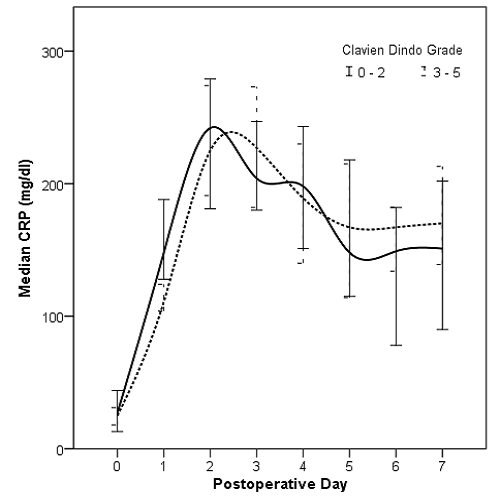
\includegraphics[width=\textwidth]{../Figures/crp_comp_infective_leak1}
			\\ Patients with POPF
		\end{figure}
	\end{columns}
\end{frame}

\begin{frame}
	\frametitle{Receiver operating characteristics analysis}
	\framesubtitle{CRP thresholds for predicting infective complications in the absence of a POPF. }
	\begin{columns}
		\column[c]{0.45\textwidth}
			\begin{figure}
				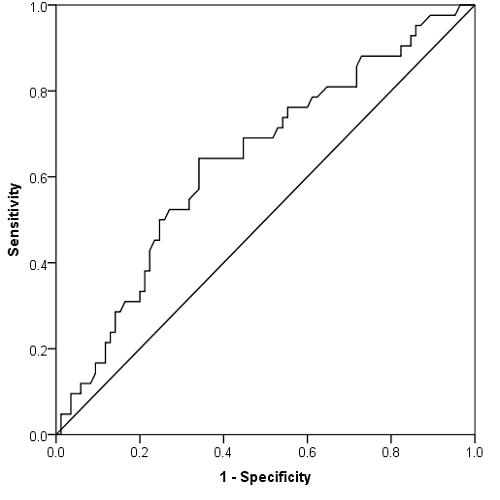
\includegraphics[width=\textwidth]{../Figures/crp_comp_ROC_infection_D3}
				\\{\scriptsize D3 178 mg/dl; AUC 0.64; NPV 0.79; \\Spec 0.66; Sens 0.64; p=0.011}
			\end{figure}
		
		\column[c]{0.45\textwidth}
			\begin{figure}
				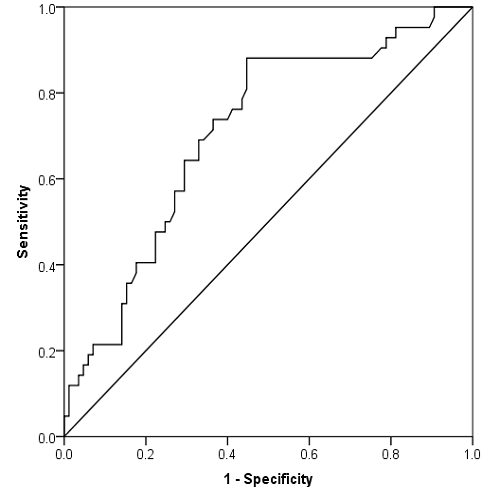
\includegraphics[width=\textwidth]{../Figures/crp_comp_ROC_infection_D4}
				\\{\scriptsize D4 125 mg/dl; AUC 0.71; NPV 0.83; \\Spec 0.64; Sens 0.74; p$<$0.001}
			\end{figure}
	\end{columns}
\end{frame}



\section[Chapter 7]{Discussion}
\begin{frame}
	\frametitle{Future directions}
	\begin{itemize}
		\item Assessing impact of prehabilitation
		\item Improving in aerobic capacity and body composition through nutritional supplementation and physical exercise
		\item Assessing impact of neo-adjuvant treatments
		\item Customising goal-directed therapy based on CPET
		\item Correction of anaemia through preoperative iron supplementation
		\item Early recognition and aggressive management of complications
		\item Assessing suitability for 'fast-track' to surgery and 'enhanced-recovery'
	\end{itemize}
\end{frame}


\section{Case study}
\begin{frame}
	\frametitle{A case study}
	\framesubtitle{How does this work influence decision-making?}
	\begin{itemize}
		\item 63 yr old female with BMI of 35 presents with painless OJ
		\item PMH - HTN, T2DM, ex-smoker
		\item Bloods: Bil 180, CRP 22, Alb 30
		\item Imaging: Resectable tumour of head of pancreas
		\medskip \hrule \medskip
\pause
		\item Should this patient undergo CPET?
		\item Should this patient undergo biliary drainage?
		\item Should we wait until resolution of jaundice before CPET?
		\item How can the CPET results be used to influence her care?
		\item How can the postoperative inflammatory markers be used to manage her care?
	\end{itemize}
\end{frame}

\begin{frame}
	\frametitle{A case study}
	\begin{description}
	{\scriptsize 	
		\item [Chapter 2] CPET may allow identifying if she is at increased risk of complications, prolonged hospital stay and non-receipt of adjuvant therapy. 
					\\ CPET should not be used on its own to decline surgery. 
					\hrule
\pause
		\item [Chapter 3] CPET can be performed in the presence of jaundice. 
					\\ Jaundice does not adversely affect dynamic cardiopulmonary response to and this cannot be a justification for biliary drainage. 
					\\ Taken together with evidence from trials on preperative biliary drainage, she should proceed direct to surgery.
						\hrule
\pause
		\item [Chapter 4] Interpret low $\dot{V}_{O_2}$ in her case with caution. 
					\\ Her aerobic capacity may be better than that suggested by her results. 
					\\ Beware of \textit{spurious correlation} with total body weight.
						\hrule
\pause
		\item [Chapter 5] Jaundice and hypo-albuminemia attenuate post-op inflammatory response.
					\\ However, this does not translate into increased complications. 
					\\ Aerobic capacity does not affect post-op inflammatory response.
						\hrule
\pause
		\item [Chapter 6] If her drain amylase on D3 is normal and D3 CRP$<$178 or D4 CRP$<$125, she is likely to have an uneventful postoperative course and must continue on 'enhanced-recovery' pathway.
				\\ If she develops a POPF, the early inflammatory response does not predict outcome.
	}
	\end{description}
\end{frame}

\begin{frame}
\centerline{Thank You}
\end{frame}


\begin{frame}
\frametitle{Tools and Roles}
%\framesubtitle{Tools and Roles}

\begin{table}
	\begin{tabular}{r l}
		        database & MS Access with VBA            \\
		data collection: & VBA + Dynamic Data Exchange   \\
		     statistics: & SPSS versions 19, 22          \\
		   bibliography: & Zotero, Bibus                 \\
		 thesis writing: & LaTeX using TeXstudio         \\
		version control: & Git + Dropbox                 \\
		                 &  \\
		         salary: & Surgical Critical Care Fellow \\
		                 & Surgical SpR on-call at GRI   \\
		                 & \\
		         sanity: & Staff on Surgical HDU, Donny
	\end{tabular}
\end{table}




\end{frame}

%----------------------------------------------------------------------------------------

\end{document} 